\documentclass[tikz,border=3pt]{standalone}
\usepackage[utf8]{inputenc}
\usepackage[T1]{fontenc}
\usepackage{lmodern}
\renewcommand{\familydefault}{\sfdefault}
\usepackage{sansmath}\sansmath
\usepackage{chemfig}
\usepackage{pgfplots}\pgfplotsset{compat=1.18,/pgf/number format/use comma,/pgf/number format/1000 sep={.}}
\usetikzlibrary{arrows.meta,calc,positioning,decorations.pathmorphing,patterns}
% paleta del sitio
\definecolor{nar}{HTML}{E8680C}\definecolor{narc}{HTML}{FFB35C}\definecolor{hielo}{HTML}{FFF3E8}
\definecolor{tinta}{HTML}{1D1D1F}\definecolor{gris}{HTML}{6E6E73}\definecolor{lila}{HTML}{7C5CF0}
\definecolor{azul}{HTML}{2F6FD6}\definecolor{menta}{HTML}{17A673}\definecolor{coral}{HTML}{E8342A}
\begin{document}
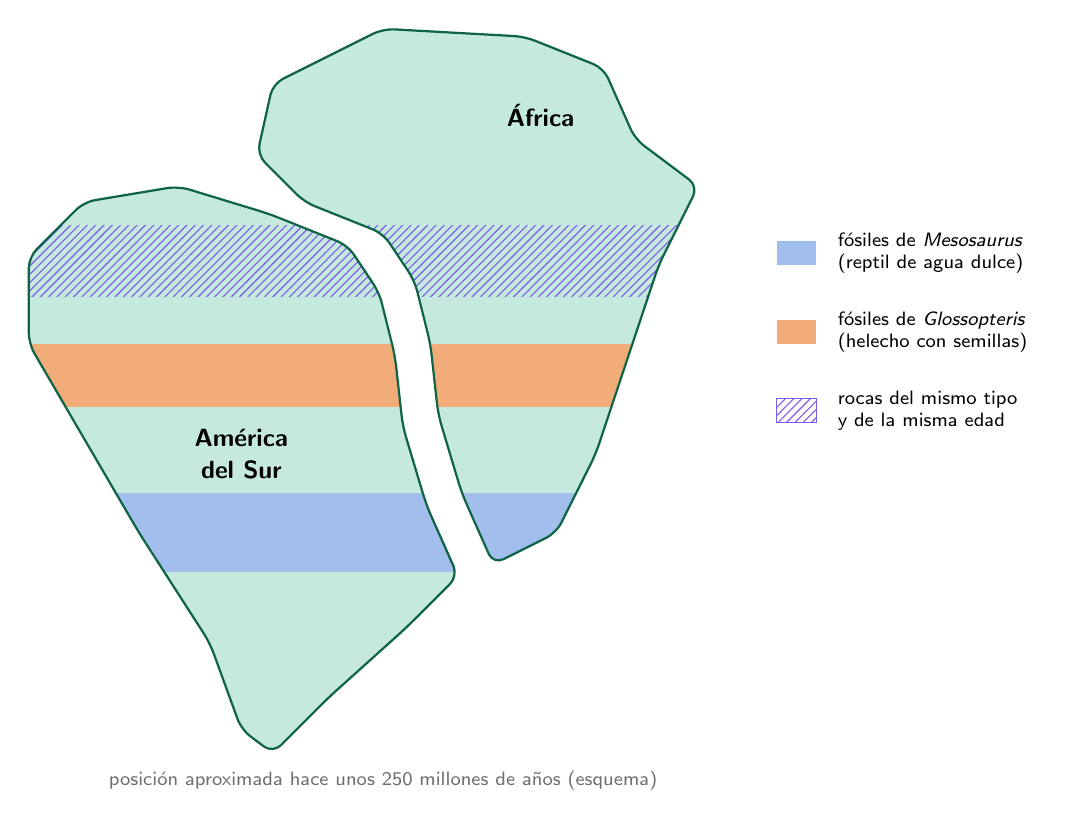
\begin{tikzpicture}[font=\footnotesize,>={Stealth[length=2.2mm]}]
\def\africa{(0.2,2.4) -- (-0.4,3.0) -- (-0.2,3.9) -- (1.2,4.6) -- (3.0,4.5) -- (4.0,4.1) -- (4.4,3.2) -- (5.2,2.6) -- (4.7,1.6) -- (4.3,0.4) -- (3.9,-0.8) -- (3.4,-1.8) -- (2.6,-2.2) -- (2.2,-1.3) -- (1.9,-0.3) -- (1.8,0.6) -- (1.6,1.4) -- (1.2,2.0) -- cycle}
\def\sudam{(-0.25,2.25) -- (0.75,1.85) -- (1.15,1.25) -- (1.35,0.45) -- (1.45,-0.45) -- (1.75,-1.45) -- (2.15,-2.35) -- (1.5,-3.0) -- (0.5,-3.9) -- (-0.2,-4.6) -- (-0.6,-4.3) -- (-1.0,-3.2) -- (-1.9,-1.8) -- (-2.6,-0.6) -- (-3.3,0.6) -- (-3.3,1.7) -- (-2.6,2.4) -- (-1.4,2.6) -- cycle}
\fill[menta!25,rounded corners=4pt] \africa;
\fill[menta!25,rounded corners=4pt] \sudam;
% bandas de evidencias, recortadas a cada continente
\newcommand\bandas{
  \fill[azul!45] (-4,-2.3) rectangle (6,-1.3);
  \fill[nar!55] (-4,-0.2) rectangle (6,0.6);
  \fill[pattern=north east lines,pattern color=lila] (-4,1.2) rectangle (6,2.1);}
\begin{scope}\clip[rounded corners=4pt] \africa; \bandas \end{scope}
\begin{scope}\clip[rounded corners=4pt] \sudam; \bandas \end{scope}
\draw[menta!60!black,thick,rounded corners=4pt] \africa;
\draw[menta!60!black,thick,rounded corners=4pt] \sudam;
\node[font=\small\bfseries] at (3.2,3.5) {África};
\node[font=\small\bfseries] at (-0.6,-0.6) {América};
\node[font=\small\bfseries] at (-0.6,-1.0) {del Sur};
% leyenda
\begin{scope}[xshift=6.2cm,yshift=1.6cm]
\fill[azul!45] (0,0) rectangle (0.5,0.3); \node[anchor=west,align=left,font=\scriptsize] at (0.65,0.15) {fósiles de \textit{Mesosaurus}\\(reptil de agua dulce)};
\fill[nar!55] (0,-1.0) rectangle (0.5,-0.7); \node[anchor=west,align=left,font=\scriptsize] at (0.65,-0.85) {fósiles de \textit{Glossopteris}\\(helecho con semillas)};
\fill[pattern=north east lines,pattern color=lila] (0,-2.0) rectangle (0.5,-1.7); \draw[lila] (0,-2.0) rectangle (0.5,-1.7);
\node[anchor=west,align=left,font=\scriptsize] at (0.65,-1.85) {rocas del mismo tipo\\y de la misma edad};
\end{scope}
\node[font=\scriptsize,text=gris,anchor=north] at (1.2,-4.7) {posición aproximada hace unos 250 millones de años (esquema)};
\end{tikzpicture}
\end{document}
